\chapter{Analisis}
\label{chap:analisi}

%Analisis Aplikasi Sejenis
\section{Analisis Aplikasi Sejenis}
\label{lab:Analisis Aplikasi Sejenis}
% Aplikasi publik transport Android
\hspace{0.5cm} Aplikasi sejenis penulis temui bernama "Public Transport". Namun aplikasi tersebut hanya dapat dijalankan di sistem aplikasi android. Aplikasi "Public Transport" ini memanfaatkan Kiri API. Penggunaannya cukup sederhana. Di halaman awal pengguna dapat mengetikan lokasi awal dan tujuan. Selain dengan mengetik pengguna juga dapat menunjuk lokasi pada peta. Setelah lokasi dipilih sistem akan memastikan dengan memberi daftar nama jalan dan tempat terkait. Jika sudah memilih maka sistem akan mengeluarkan hasil pencarian rute.

Berikut adalah tampilan dari aplikasi "Public Transport" (Gambar ~\ref{fig:home} sampai ~\ref{fig:peta}):

\begin{figure}[h]
	\centering
		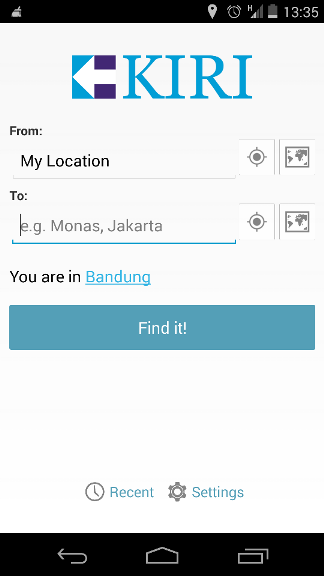
\includegraphics[scale=0.5]{Gambar/KIRI_Android/home}
	\caption{Tampilan awal aplikasi Public Transport}
	\label{fig:home}
\end{figure}

\begin{figure}[h]
	\centering
		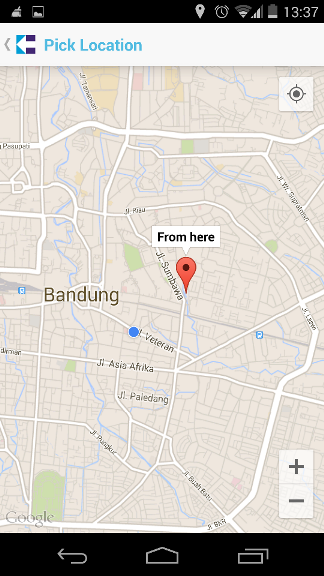
\includegraphics[scale=0.5]{Gambar/KIRI_Android/menunjuk_lokasi}
	\caption{Menunjuk lokasi pada peta}
	\label{fig:menunjuk}
\end{figure}

\begin{figure}[h]
	\centering
		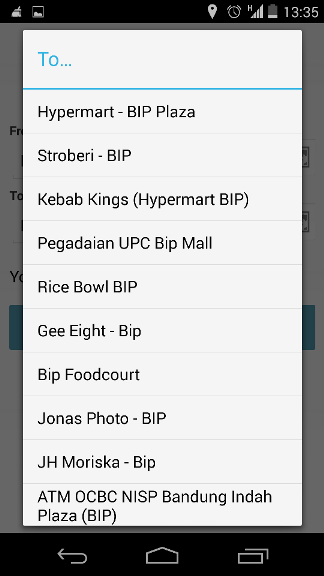
\includegraphics[scale=0.5]{Gambar/KIRI_Android/terkait}
	\caption{Memberikan daftar nama tempat dan nama jalan terkait}
	\label{fig:terkait}
\end{figure}

\begin{figure}[h]
	\centering
		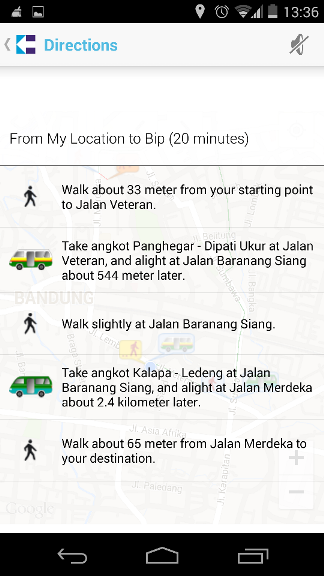
\includegraphics[scale=0.5]{Gambar/KIRI_Android/tampilan_daftar}
	\caption{Tampilan rute kendaraan umum dalam bentuk daftar}
	\label{fig:daftar}
\end{figure}

\begin{figure}[h]
	\centering
		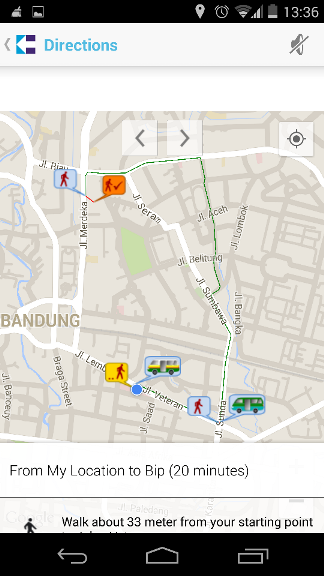
\includegraphics[scale=0.5]{Gambar/KIRI_Android/tampilan_peta}
	\caption{Tampilan rute kendaraan umum di peta}
	\label{fig:peta}
\end{figure}
% tampilannya, cara kerja, hal yang dapat dilakukan

\clearpage

%Analisis Analisis Program
\section{Analisis Aplikasi}
\label{lab:Analisis Aplikasi}
\hspace{0.5cm} Aplikasi akan dibuat mengguakan bahasa pemograman C\#. Aplikasi yang digunakan untuk membangun Aplikasi Pencari Rute Kendaraan Umum untuk Windows Phone adalah Visual Studio Express 2013. Pada sub bab ini akan dibahas diagram use case dan diagram kelas dari aplikasi yang akan dibangun. 

%Analisis Kebutuhan Aplikasi
\subsection{Kebutuhan Aplikasi}
\label{lab:Kebutuhan Aplikasi}

% SUB Analisis Kontrol yang Dipakai
\subsection{Analisis Kontrol yang Dipakai}
\label{lab:Analisis Kontrol yang Dipakai}

% SUB Analisis Terhadap Siklus Hidup Aplikasi
\subsection{Analisis Terhadap Siklus Hidup Aplikasi}
\label{lab:Analisis Terhadap Siklus Hidup Aplikasi}

% SUB Analisis Peta
\subsection{Analisis Peta}
\label{lab:Analisis Peta}

% SUB Analisis Metode yang Dipakai
\subsection{Analisis Metode yang Dipakai}
\label{lab:Analisis Metode yang Dipakai}


%Analisis Diagram Use-Case dan Scenario
\subsection{Diagram Use-Case dan Scenario}
\label{lab:Diagram Use-Case dan Scenario}
\hspace{0.5cm} Diagram use-case adalah diagram yang menjelaskan interaksi sistem dengan lingkungan (contoh: pengguna). Berdasarkan analisa di atas maka pengguna dapat:
\begin{itemize}
	\item Mendapatkan lokasi pengguna berada.
	\item Memasukan lokasi asal.
	\item Memasukan lokasi lokasi tujuan.
	\item Menunjuk langsung lokasi asal dan tujuan pada peta.
	\item Memilih alamat atau tempat dari pilihan yang disediakan.
	\item Melihat rute kendaraan umum dalam bentuk titik dan \textit{pushpin} pada peta atau bentuk daftar dari tempat asal ke tempat tujuan.
\end{itemize}

Berikut adalah diaram use case saat pengguna mencari rute kendaraan umum (Gambar:~\ref{fig:UseCase}):
% Use case
\begin{figure}[h]
	\centering
		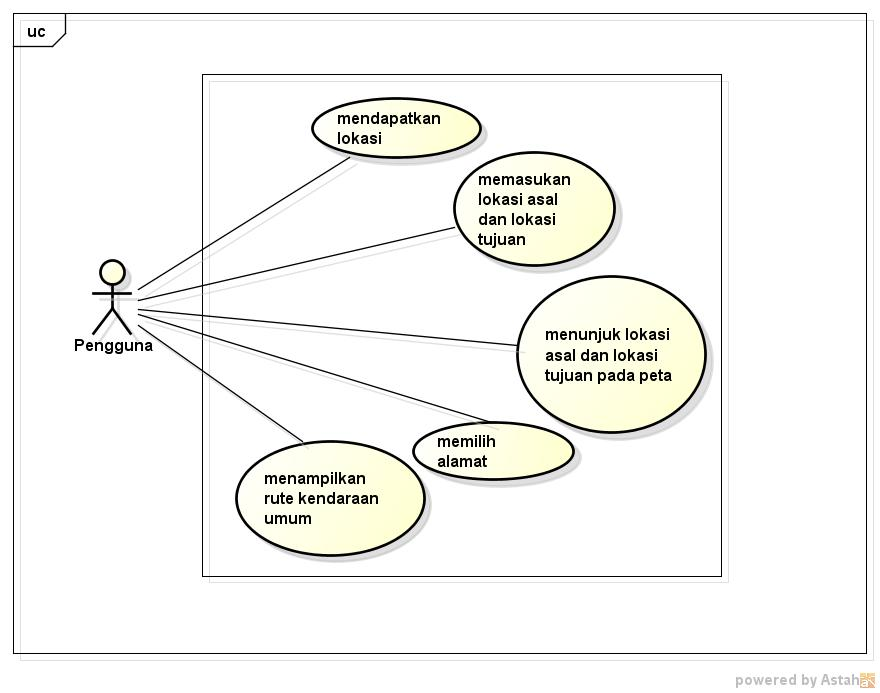
\includegraphics[scale=0.5]{Gambar/useCase_dan_Class/UseCase}
	\caption{Diagram Use Case}
	\label{fig:UseCase}
\end{figure}

% Skenario Melakukan pencarian rute 
\textbf{Skenario melakukan pencarian rute kendaraan umum}
Nama: Mencari rute kendaraan umum
Aktor: Pengguna
Kondisi Awal: Perangkat lunak dijalankan dan pengguna tidak tahu harus memakai kendaraan umum apa
Deskripsi: Pengguna memasukan lokasi awal dan lokasi tujuan
Kondisi akhir: Aplikasi memberitahukan kendaraan umum yang harus dinaiki pengguna.
Skenario:
\begin{enumerate}
	\item Pengguna memasukan lokasi awal dan tujuan atau menuntuk langsung pada peta.
	\item Sistem memberikan daftar tempat atau jalan terkait.
	\item Pengguna memilih dari daftar tempat atau jalan terkait.
	\item Sistem menentukan rute terbaik.
	\item Sistem menampilkan rute dalam 2 bentuk yaitu daftar dan titik pada peta.
\end{enumerate}
Eksepsi:
\begin{enumerate}
	\item Pengguna memasukan lokasi yang tidak terdaftar di sistem.
	\item Sistem memberi notifikasi bahwa lokasi tidak ditemukan.
\end{enumerate}

%Analisis Class Diagram
\subsection{Class Diagram}
\label{lab:Class Diagram}